\section{Durchführung}
\label{sec:Durchführung}
\subsection{Inbetriebnahme des Laser}
Zur Beginn des Versuches werden zunächst die Laserdiode, sowie die Absorptionszelle mit dem Rubidium und ein Detektor justiert. Außerdem wird eine Temperatur von $T=\SI{50}{\degreeCelsius}$ am Laserkontrollgerät eingestellt und die Apparatur wird aufgeheizt. Da der Laserstrahl mit dem menschlichen Auge nicht zu sehen ist,
muss zur Justage eine Infrarot Karte benutzt werden.
Um sicherzustellen, dass der Laserstrahl die Absorptionszelle und den Detektor exakt trifft, wird mithilfe der IR-Karte der Laser sichtbar gemacht und per Kamera beobachtet. Der Aufbau ist in in Abbildung (\ref{fig:auf1}) dargestellt.
\begin{figure}[h!]
  \centering
  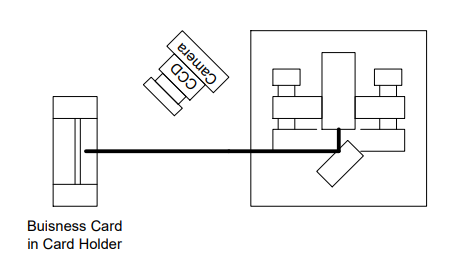
\includegraphics[scale=0.7]{fig/auf1.png}
  \caption{Sichtbar machen des Laser durch IR-Karte \cite[6]{Anleitung4}.}
  \label{fig:auf1}
\end{figure}
\FloatBarrier
\noindent Jetzt wird der Strom solange erhöht bis sogenannte Speckle auf der IR-Karte sichtbar werden. Sobald diese erscheinen ist der Schwellenstrom erreicht und die Diode arbeitet im Laserbetrieb.
\subsection{Bestimmung der Absorptionswellenlänge}
Der Laser ist nun justiert, die Kamera wird auf die Rubidiumzelle ausgerichtet. Anschließend wird das Licht gedimmt, um den Einfluss von Hintergrundlicht auf die Photodiode, die als Detektor dient, zu minimieren. Ebenfalls muss die Intensität des Laserstrahl durch Neutralfilter reduziert werden, da sonst ebenfalls die Photodiode gesättigt wäre. Das Laserkontrollgerät wird mit einem Oszilloskop verbunden.
In Abbildung (\ref{fig:auf2}) ist die verwendete Verkabelung dargestellt.
\begin{figure}[h!]
  \centering
  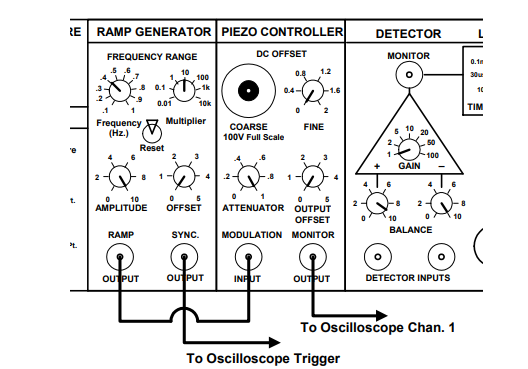
\includegraphics[scale=0.7]{fig/auf2.png}
  \caption{Verkabelung des Kontrollgeräts \cite[10]{Anleitung4}.}
  \label{fig:auf2}
\end{figure}
\FloatBarrier
\noindent Beim Ramp-Generator wird die Frequenz auf $\SI{10}{\hertz}$ gestellt, sodass eine Dreieckswelle entsteht mit ausreichend großer Amplitude. Jetzt wird der Strom so justiert, dass die
Rubidiumzelle Licht emittiert. Damit ist die richtige Frequenz gefunden und ein Foto der Rubidiumzelle wird aufgenommen.
In Abbildung (\ref{fig:auf3}) ist der Experimentaufbau dafür schematisch dargestellt.
\begin{figure}[h!]
  \centering
  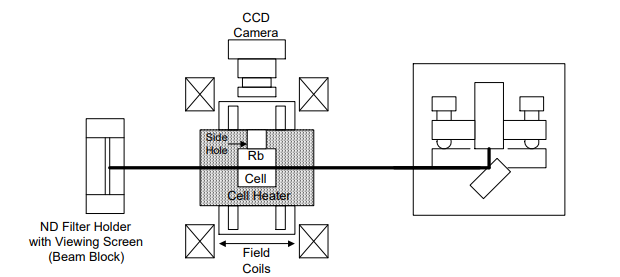
\includegraphics[scale=0.7]{fig/auf3.png}
  \caption{Aufbau zur Bestimmung der Absorptionswellenlänge \cite[9]{Anleitung4}.}
  \label{fig:auf3}
\end{figure}
\FloatBarrier
\subsection{Bestimmung des Absorptionsspektrum}
Um die Modensprünge zu eliminieren wird die Verkabelung wie in Abbildung (\ref{fig:auf4}) geändert.
\begin{figure}[h!]
  \centering
  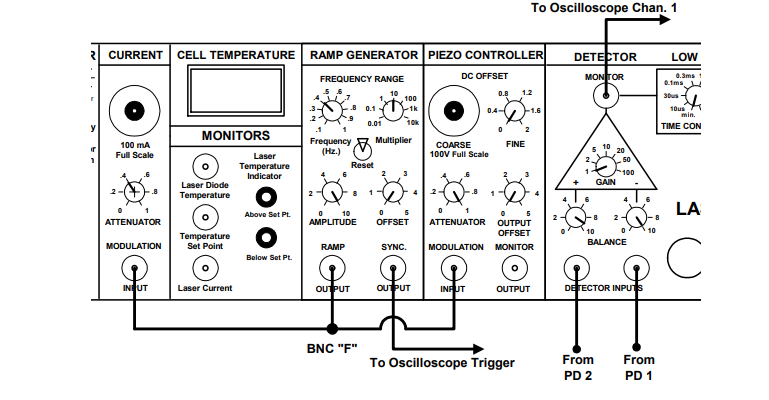
\includegraphics[scale=0.5]{fig/auf4.png}
  \caption{Verkabelung zur Bestimmung des Absorptionsspektrum \cite[16]{Anleitung4}.}
  \label{fig:auf4}
\end{figure}
\FloatBarrier
\noindent Ebenfalls wird eine zweite Photodiode hinzugefügt und ein 50/50 Strahlteiler wird vor die Rubidiumzelle gesetzt. Das Experiment sieht jetzt aus wie in Abbildung (\ref{fig:auf5}).
\begin{figure}[h!]
  \centering
  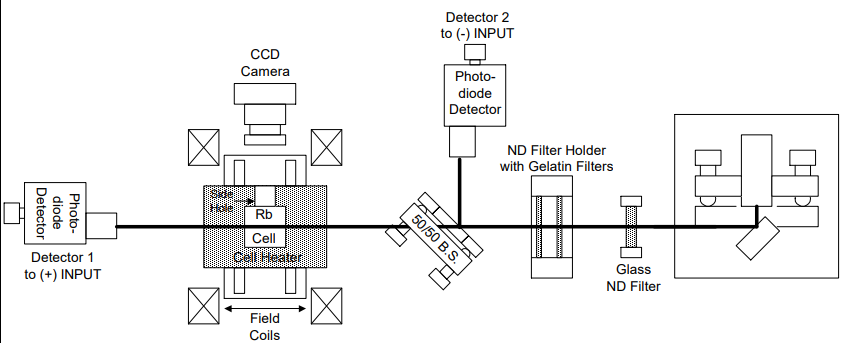
\includegraphics[scale=0.5]{fig/auf5.png}
  \caption{Aufbau zur Bestimmung des Absorptionsspektrum \cite[16]{Anleitung4}.}
  \label{fig:auf5}
\end{figure}
\FloatBarrier
\noindent Als letztes wird nun solange mit den verschiedenen Reglern am Laserkontrollgerät nachjustiert, bis das Absorptionsspektrum vernünftig zu sehen ist und ein Foto aufgenommen werden kann.
